%%%%%%%%%%%%%%%%%%%%%%%%%%%%%%%%%%%%%%%%%%%%%%%%%%%%%%%%%%%%%%%%%%%%%%
%%                     delay
%%%%%%%%%%%%%%%%%%%%%%%%%%%%%%%%%%%%%%%%%%%%%%%%%%%%%%%%%%%%%%%%%%%%%%
\color{red}
\subsection{Glyph: \glyph{delay}}\label{sec:delay}

The glyph \glyph{delay} is used to denote that the \glyph{interactor} linked as input does not produce the influence immediately.

\begin{glyphDescription}
 \glyphSboTerm SBO:NEW ! delay.
 \glyphOrigin One interactor (section~\ref{sec:interactors}) or logical operator (section~\ref{sec:logic}).
 \glyphTarget  One modulation (section~\ref{sec:modulation}), stimulation (section~\ref{sec:stimulation}), inhibition (section~\ref{sec:inhibition}), necessary  stimulation (section~\ref{sec:necessaryStimulation}), or absolute inhibition (section~\ref{sec:absoluteInhibition}) arc.
 \glyphNode \glyph{Not} is represented by a circle carrying the greek letter ``\tau`` (``TAU'').
 \end{glyphDescription}

\begin{figure}[H]
  \centering
  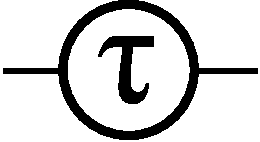
\includegraphics[scale = 0.5]{images/delay}
  \caption{The \ER glyph for \glyph{delay}.}
  \label{fig:not}
\end{figure}

